\documentclass[11pt]{article}
\usepackage[notes]{la}
\lamodule{4}{1}{Vector Spaces and Subspaces}
\laxdoc{1.2}
\laxdoc{1.3}
\laxdoc{1.4}
\laxdoc{1.5}
\laxdoc{1.7}
\laxdoc{2.1}
\laxdoc{3.2}

\begin{document}

\section{Vector Spaces and Subspaces}

\begin{guide}
Until now a ``vector'' meant a list of $n$ numbers. But you have already added and scaled other kinds of objects: polynomials (Section 1.7), matrices (Section 2.1), and functions in calculus. Do these obey the same algebra as $\R^n$? Which properties of $\R^n$ did we \emph{really} use, and what happens if we keep those properties and throw away everything else, in particular the idea that a vector is a column of numbers? Whatever we then prove will hold for lists, polynomials, matrices and functions all at once.
\end{guide}

\textbf{By the end of this section you should be able to:}
\begin{itemize}
  \item state the ten axioms of a vector space, and identify the typical vector, the sum, the scalar multiple, the zero vector and the negative of a vector in $\R^n$, in spaces of polynomials, in spaces of matrices and in spaces of functions;
  \item prove elementary facts directly from the axioms (the zero vector is unique, $0\bv{u}=\bv{0}$, $c\bv{0}=\bv{0}$, $(-1)\bv{u}=-\bv{u}$);
  \item decide whether a set with given operations is a vector space, and say \emph{exactly which axiom fails} when it is not;
  \item state and use the Subspace Test, and either prove that a subset is a subspace or disprove it with specific vectors;
  \item recognise a set described by a parametric formula as a span, rewrite a set described by a restriction as a span, and prove that every span is a subspace;
  \item decide whether a polynomial, a matrix or a function lies in a given span by solving a linear system from Chapter 1.
\end{itemize}

% ---------------------------------------------------------------------
\subsection*{One algebra, many worlds}

Look at four calculations that you could do right now.
\begin{itemize}
  \item In $\R^3$: $(1,2,3)+(4,0,-1)=(5,2,2)$ and $2(1,2,3)=(2,4,6)$.
  \item With polynomials of degree at most $2$: $(1+2t+3t^2)+(4-t^2)=5+2t+2t^2$ and $2(1+2t+3t^2)=2+4t+6t^2$.
  \item With $2\times2$ matrices (Definition~\ref{2.1-def:sum}): $\begin{bmatrix}1&2\\3&4\end{bmatrix}+\begin{bmatrix}0&-1\\5&2\end{bmatrix}=\begin{bmatrix}1&1\\8&6\end{bmatrix}$ and $2\begin{bmatrix}1&2\\3&4\end{bmatrix}=\begin{bmatrix}2&4\\6&8\end{bmatrix}$.
  \item With functions: if $f(t)=\sin t$ and $g(t)=t^2$, then $(f+g)(t)=\sin t+t^2$ and $(2f)(t)=2\sin t$.
\end{itemize}
Each time, two objects of one kind are combined into another object of the \emph{same} kind, and a number scales an object of that kind. In Section 1.3 we listed eight rules for $\R^n$ (Theorem~\ref{1.3-thm:props}), and Pause and think~\ref{1.3-think:axioms} asked which rules a different world of ``vectors'' would have to satisfy. This section answers that question: any collection of objects with a sum and a scalar multiple that obey the right list of rules deserves to be called a \emph{vector space}, and everything we know about combining vectors will carry over.

\begin{kc}{Adding and scaling in new worlds}{newworlds}
Compute: (a)~$(2+t-t^2)+(1-3t+4t^2)$ in the space of polynomials of degree at most $2$; (b)~$3\begin{bmatrix}1&0\\2&-1\end{bmatrix}-\begin{bmatrix}0&1\\1&1\end{bmatrix}$ in the space of $2\times2$ matrices; (c)~$f-2g$ if $f(t)=1+t$ and $g(t)=t^2$, as a formula in $t$, and its value at $t=2$ computed in two ways.
\end{kc}

\begin{think}{Which properties did we really use?}{used}
In Chapters 1 to 3 we proved many things about linear combinations. Think of one argument from those chapters that used only the \emph{rules} of addition and scaling (for instance the argument that a sum of two linear combinations of $\bv{w}_1,\bv{w}_2,\bv{w}_3$ is again a linear combination of them, Pause and think~\ref{1.3-think:closure}), and one computation that used the \emph{entries} of a vector (for instance row reduction). Which of the two kinds of argument could be repeated for polynomials or functions word for word, and which could not?
\end{think}

% ---------------------------------------------------------------------
\subsection*{The definition}

\begin{defn}{Vector space}{vspace}
A \emph{vector space} is a nonempty set $V$ of objects, called \emph{vectors}, on which two operations are defined, \emph{addition} (any two vectors $\bv{u},\bv{v}$ have a sum $\bv{u}+\bv{v}$) and \emph{multiplication by scalars} (any real number $c$ and any vector $\bv{u}$ have a scalar multiple $c\bv{u}$), such that the following ten axioms hold for all vectors $\bv{u},\bv{v},\bv{w}$ in $V$ and all scalars $c,d$.

\textbf{Closure.}
\begin{itemize}[label={},itemsep=1pt,leftmargin=1.5em]
  \item \textbf{(1)}~ The sum $\bv{u}+\bv{v}$ is in $V$.
  \item \textbf{(6)}~ The scalar multiple $c\bv{u}$ is in $V$.
\end{itemize}
\textbf{Addition.}
\begin{itemize}[label={},itemsep=1pt,leftmargin=1.5em]
  \item \textbf{(2)}~ $\bv{u}+\bv{v}=\bv{v}+\bv{u}$.
  \item \textbf{(3)}~ $(\bv{u}+\bv{v})+\bv{w}=\bv{u}+(\bv{v}+\bv{w})$.
  \item \textbf{(4)}~ There is a vector $\bv{0}$ in $V$, the \emph{zero vector}, with $\bv{u}+\bv{0}=\bv{u}$ for every $\bv{u}$.
  \item \textbf{(5)}~ For each $\bv{u}$ there is a vector $-\bv{u}$ in $V$, the \emph{negative} of $\bv{u}$, with $\bv{u}+(-\bv{u})=\bv{0}$.
\end{itemize}
\textbf{Scalar multiplication.}
\begin{itemize}[label={},itemsep=1pt,leftmargin=1.5em]
  \item \textbf{(7)}~ $c(\bv{u}+\bv{v})=c\bv{u}+c\bv{v}$.
  \item \textbf{(8)}~ $(c+d)\bv{u}=c\bv{u}+d\bv{u}$.
  \item \textbf{(9)}~ $c(d\bv{u})=(cd)\bv{u}$.
  \item \textbf{(10)}~ $1\bv{u}=\bv{u}$.
\end{itemize}
\end{defn}

The numbering is the one used in Lay's textbook. How do the axioms relate to what we know? Axioms (2), (3), (4), (5), (7), (8), (9), (10) are exactly the eight rules (i) to (viii) of Theorem~\ref{1.3-thm:props}, so $\R^n$ satisfies them; the closure axioms (1) and (6) hold because adding two lists of $n$ numbers, or scaling one, gives another list of $n$ numbers. Hence \textbf{$\R^n$ is a vector space}, for every $n\geq1$. We now read the axioms as three groups of requirements.
\begin{itemize}
  \item \emph{Closure} is a requirement on the \emph{set}: the operations must never take you out of $V$.
  \item The \emph{addition} axioms say that the sum behaves like the sum of numbers: the order and the grouping do not matter, there is a vector that changes nothing, and every vector can be cancelled.
  \item The \emph{scalar} axioms say how scaling interacts with addition of vectors (7), with addition of scalars (8), with multiplication of scalars (9), and that the scalar $1$ does nothing (10).
\end{itemize}

\begin{remark}[The zero vector is part of the structure]
Axiom (4) does not say ``the number $0$ is a vector''. It says that $V$ \emph{contains a vector called $\bv{0}$} that behaves as a zero for addition. Which vector that is depends on the space: it is $(0,0,0)$ in $\R^3$, the zero polynomial in a space of polynomials, the zero matrix in a space of matrices and the function that is $0$ for every input in a space of functions. The bold $\bv{0}$ is a vector; the plain $0$ is a scalar. When we study a new set with new operations, finding its zero vector is the first thing to do, and sometimes it is not what you expect: if the positive real numbers are given the ``sum'' $x\oplus y=xy$ (the ordinary product), then the zero vector is the number $1$, because $x\oplus1=x$.
\end{remark}

% ---------------------------------------------------------------------
\subsection*{First consequences of the axioms}

For numbers nobody asks for a proof of $0\cdot x=0$. In a general vector space we may not use entries, so every fact must come from the ten axioms alone.

\begin{thm}{First consequences of the axioms}{conseq}
Let $V$ be a vector space, $\bv{u}$ a vector in $V$ and $c$ a scalar.
\begin{enumerate}[label=(\alph*),itemsep=1pt]
  \item The zero vector is unique: if $\bv{z}$ is a vector with $\bv{u}+\bv{z}=\bv{u}$ for all $\bv{u}$ in $V$, then $\bv{z}=\bv{0}$.
  \item The negative is unique: if $\bv{u}+\bv{w}=\bv{0}$, then $\bv{w}=-\bv{u}$.
  \item $0\bv{u}=\bv{0}$.
  \item $c\bv{0}=\bv{0}$.
  \item $(-1)\bv{u}=-\bv{u}$.
\end{enumerate}
\end{thm}

\begin{proof}
Write ``(A$k$)'' for axiom $(k)$.

(a)~Taking $\bv{u}=\bv{0}$ in $\bv{u}+\bv{z}=\bv{u}$ gives $\bv{0}+\bv{z}=\bv{0}$. By (A2) and (A4), $\bv{0}+\bv{z}=\bv{z}+\bv{0}=\bv{z}$. Hence $\bv{z}=\bv{0}$.

(b)~By (A2), $(-\bv{u})+\bv{u}=\bv{u}+(-\bv{u})=\bv{0}$ (A5), and by (A2) and (A4), $\bv{0}+\bv{w}=\bv{w}+\bv{0}=\bv{w}$. So
\[
\bv{w}=\bv{0}+\bv{w}=\bigl((-\bv{u})+\bv{u}\bigr)+\bv{w}=(-\bv{u})+(\bv{u}+\bv{w})=(-\bv{u})+\bv{0}=-\bv{u},
\]
where the third equality is (A3), the fourth uses $\bv{u}+\bv{w}=\bv{0}$, and the last is (A4).

(c)~Put $\bv{w}=0\bv{u}$. By (A8), $\bv{w}=(0+0)\bv{u}=0\bv{u}+0\bv{u}=\bv{w}+\bv{w}$. Then
\[
\bv{0}=\bv{w}+(-\bv{w})=(\bv{w}+\bv{w})+(-\bv{w})=\bv{w}+\bigl(\bv{w}+(-\bv{w})\bigr)=\bv{w}+\bv{0}=\bv{w},
\]
by (A5), the equation $\bv{w}=\bv{w}+\bv{w}$, (A3), (A5) and (A4). So $0\bv{u}=\bv{0}$.

(d)~Put $\bv{w}=c\bv{0}$. By (A4), $\bv{0}+\bv{0}=\bv{0}$, so by (A7), $\bv{w}=c(\bv{0}+\bv{0})=c\bv{0}+c\bv{0}=\bv{w}+\bv{w}$. The computation in~(c) then gives $\bv{w}=\bv{0}$.

(e)~By (A10), (A8) and part~(c),
\[
\bv{u}+(-1)\bv{u}=1\bv{u}+(-1)\bv{u}=\bigl(1+(-1)\bigr)\bv{u}=0\bv{u}=\bv{0}.
\]
Part~(b) with $\bv{w}=(-1)\bv{u}$ shows $(-1)\bv{u}=-\bv{u}$.
\end{proof}

Notice what the proof does \emph{not} do: it never looks inside a vector. That is the point. These facts hold in every vector space, including ones nobody has invented yet.

\begin{kc}{Which axiom?}{axiomsteps}
Here is a proof of the cancellation law: if $\bv{u}+\bv{w}=\bv{v}+\bv{w}$, then $\bv{u}=\bv{v}$. Name the axiom, or the hypothesis, that justifies each equality.
\[
\bv{u}=\bv{u}+\bv{0}=\bv{u}+\bigl(\bv{w}+(-\bv{w})\bigr)=(\bv{u}+\bv{w})+(-\bv{w})=(\bv{v}+\bv{w})+(-\bv{w})=\bv{v}+\bigl(\bv{w}+(-\bv{w})\bigr)=\bv{v}+\bv{0}=\bv{v}.
\]
\end{kc}

\begin{think}{Why prove what is obvious?}{prove}
For numbers, $0\cdot x=0$ is something everyone ``knows''. Why should we bother to prove $0\bv{u}=\bv{0}$ from the axioms? Could $0\bv{u}$ fail to be the zero vector in some system where we define a sum and a scalar multiple by our own rules, and if so, what does that tell you about how much you may assume? (The first non-example below gives you a concrete case; come back to this question after you have seen it.)
\end{think}

% ---------------------------------------------------------------------
\subsection*{Examples of vector spaces}

The following example answers, for four spaces at once, the questions that you must be able to answer about \emph{any} vector space: what does a typical vector look like, what does adding two vectors mean, what does scaling look like, what is the zero vector, and what is the negative of a vector.

\begin{exmp}{The anatomy of four vector spaces}{anatomy}
\textbf{(a) The space $\R^3$.}
\begin{itemize}[itemsep=1pt]
  \item \emph{A typical vector:} a list of three numbers, for instance $\bv{u}=(2,-1,5)$.
  \item \emph{Addition} adds entries in the same position: $(2,-1,5)+(1,4,-3)=(3,3,2)$.
  \item \emph{Scalar multiplication} multiplies every entry: $3(2,-1,5)=(6,-3,15)$.
  \item \emph{The zero vector} is $(0,0,0)$: adding it changes no entry.
  \item \emph{The negative} of $(2,-1,5)$ is $(-2,1,-5)$, which is $(-1)\bv{u}$; indeed $(2,-1,5)+(-2,1,-5)=(0,0,0)$.
\end{itemize}
\textbf{(b) The space $\mathbb{P}_2$ of polynomials of degree at most $2$.}
\begin{itemize}[itemsep=1pt]
  \item \emph{A typical vector:} a polynomial $p(t)=a_0+a_1t+a_2t^2$, for instance $p(t)=2-t+5t^2$. The vector is the \emph{polynomial}; the list $(2,-1,5)$ of its coefficients is only a way of writing it down.
  \item \emph{Addition} adds the polynomials, which means adding the coefficients of equal powers: if $q(t)=1+4t-3t^2$, then $(p+q)(t)=3+3t+2t^2$.
  \item \emph{Scalar multiplication} multiplies every coefficient: $(3p)(t)=6-3t+15t^2$.
  \item \emph{The zero vector} is the zero polynomial $0+0t+0t^2$, the polynomial whose value is $0$ for every $t$.
  \item \emph{The negative} of $p$ is $(-p)(t)=-2+t-5t^2$, and $p+(-p)$ is the zero polynomial.
\end{itemize}
(The arithmetic is the same as in~(a), which is why Section 1.7 could test polynomials for independence by looking at their coefficient vectors. But the objects are polynomials.)

\textbf{(c) The space $M_{2\times2}$ of $2\times2$ matrices.}
\begin{itemize}[itemsep=1pt]
  \item \emph{A typical vector:} a matrix, for instance $A=\begin{bmatrix}2&-1\\0&5\end{bmatrix}$.
  \item \emph{Addition} adds entries in the same position: with $B=\begin{bmatrix}1&4\\-3&2\end{bmatrix}$, $A+B=\begin{bmatrix}3&3\\-3&7\end{bmatrix}$.
  \item \emph{Scalar multiplication} multiplies every entry: $3A=\begin{bmatrix}6&-3\\0&15\end{bmatrix}$.
  \item \emph{The zero vector} is the zero matrix $\mathbf{0}=\begin{bmatrix}0&0\\0&0\end{bmatrix}$.
  \item \emph{The negative} of $A$ is $-A=\begin{bmatrix}-2&1\\0&-5\end{bmatrix}$.
\end{itemize}
\textbf{(d) The space $\mathcal{F}$ of all real-valued functions on $\R$.}
\begin{itemize}[itemsep=1pt]
  \item \emph{A typical vector:} a whole function, for instance $f(t)=\sin t$. It is \emph{one} vector, one ``point'' of the space, not a list of values.
  \item \emph{Addition} adds the functions input by input: if $g(t)=t^2+1$, then $(f+g)(t)=\sin t+t^2+1$. For example $(f+g)(0)=0+1=1=f(0)+g(0)$.
  \item \emph{Scalar multiplication} scales every output: $(3f)(t)=3\sin t$.
  \item \emph{The zero vector} is the function $z$ with $z(t)=0$ for \emph{every} real $t$.
  \item \emph{The negative} of $f$ is $(-f)(t)=-\sin t$, and $(f+(-f))(t)=0$ for every $t$.
\end{itemize}
\end{exmp}

\begin{kc}{Zero and negative}{zeroneg}
Find the zero vector and the negative of the given vector in each space. (a)~$\mathbb{P}_3$, the polynomials of degree at most $3$: $p(t)=1-t+2t^3$. (b)~$M_{2\times3}$: $A=\begin{bmatrix}1&0&-2\\3&1&4\end{bmatrix}$. (c)~The functions on the interval $[0,1]$: $f(t)=t^2$; also compute $(f+(-f))(\tfrac12)$.
\end{kc}

\begin{exmp}{Checking the axioms for polynomials and matrices}{axioms}
\textbf{The space $\mathbb{P}_n$.} Let $p(t)=a_0+a_1t+\cdots+a_nt^n$ and $q(t)=b_0+b_1t+\cdots+b_nt^n$. Then $p+q$ has coefficients $a_i+b_i$ and $cp$ has coefficients $ca_i$, and both are polynomials of degree at most $n$: axioms (1) and (6). The zero polynomial has degree at most $n$ (axiom (4)), and $(-1)p$ is in $\mathbb{P}_n$ with $p+(-1)p=\bv{0}$ (axiom (5)). Every remaining axiom compares coefficients and says something about real numbers. For instance (A8): the coefficients of $(c+d)p$ are $(c+d)a_i=ca_i+da_i$, which are the coefficients of $cp+dp$. So $\mathbb{P}_n$ is a vector space.

A numerical spot check with $p(t)=1+t$, $q(t)=2-t^2$, $c=3$, $d=-2$:
\begin{align*}
c(p+q)&=3(3+t-t^2)=9+3t-3t^2, & cp+cq&=(3+3t)+(6-3t^2)=9+3t-3t^2\ \ (\text{A7}),\\
(c+d)p&=1\cdot(1+t)=1+t, & cp+dp&=(3+3t)+(-2-2t)=1+t\ \ (\text{A8}).
\end{align*}

\textbf{The space $M_{m\times n}$.} The sum of two $m\times n$ matrices and a scalar multiple are again $m\times n$ matrices (axioms (1) and (6)); the zero matrix is the zero vector; $-A=(-1)A$ is the negative. Theorem~\ref{2.1-thm:addprops} states axioms (2), (3), (4), (7), (8) and (9) for matrices, and $1A=A$ is clear. So $M_{m\times n}$ is a vector space for all $m$ and $n$.
\end{exmp}

\begin{exmp}{Functions on an interval}{functions}
Let $\mathcal{F}[0,1]$ be the set of all real-valued functions defined on the interval $[0,1]$. Two functions are \emph{equal} when they have the same value at every $t$ in $[0,1]$. Define $(f+g)(t)=f(t)+g(t)$ and $(cf)(t)=c\,f(t)$ for each $t$.

Take $f(t)=t$ and $g(t)=1-t$. Then $(f+g)(t)=t+(1-t)=1$ for every $t$, so $f+g$ is the \emph{constant function} $1$ (not the zero function). Also $(3f)(t)=3t$, the zero vector is the function $z(t)=0$, and $(-f)(t)=-t$. Check at $t=\tfrac14$: $f(\tfrac14)+g(\tfrac14)=\tfrac14+\tfrac34=1$.

Every axiom holds because it holds \emph{at each fixed $t$}, where it is a statement about real numbers: for (A8), $((c+d)f)(t)=(c+d)f(t)=cf(t)+df(t)=(cf+df)(t)$ for every $t$, so the two functions are equal. Hence $\mathcal{F}[0,1]$ is a vector space. In exactly the same way the set of all doubly infinite sequences $(\dots,y_{-1},y_0,y_1,\dots)$, added and scaled term by term, is a vector space (Lay calls it the space of signals).
\end{exmp}

\begin{think}{One function, one vector}{function}
Let $f(t)=t$ be a function on $\R$. Then $f(0)=0$. Is $f$ the zero vector of the space of all functions on $\R$? What exactly must be true of a function for it to be the zero vector? How many numbers does it take to specify a vector in $\R^3$, and how many to specify a vector in this space?
\end{think}

\begin{exmp}{A strange scalar multiplication: which axiom fails?}{strange}
On $V=\R^2$ keep the usual addition, but define a new scalar multiplication
\[
c\odot(u_1,u_2)=(cu_1,\ u_2).
\]
This is not a vector space. Check the axioms. The sum is the usual one, so axioms (1), (2), (3), (4) with $\bv{0}=(0,0)$, and (5) hold. Axiom (6) holds since $c\odot\bv{u}$ is a vector in $\R^2$. Axiom (7) holds: $c\odot(\bv{u}+\bv{v})=(c(u_1+v_1),\,u_2+v_2)=(cu_1,u_2)+(cv_1,v_2)=c\odot\bv{u}+c\odot\bv{v}$. Axiom (9) holds: $c\odot(d\odot\bv{u})=(cdu_1,u_2)=(cd)\odot\bv{u}$. Axiom (10) holds: $1\odot\bv{u}=\bv{u}$. But \textbf{axiom (8) fails}: take $c=2$, $d=3$, $\bv{u}=(1,1)$. Then
\[
(c+d)\odot\bv{u}=5\odot(1,1)=(5,1),\qquad c\odot\bv{u}+d\odot\bv{u}=(2,1)+(3,1)=(5,2),
\]
and $(5,1)\neq(5,2)$. A single failure is enough to show that this is not a vector space. Look also at what goes wrong with Theorem~\ref{thm:conseq}(c): $0\odot(1,1)=(0,1)$, which is not the zero vector $(0,0)$. The conclusion $0\bv{u}=\bv{0}$ needs axiom (8) in its proof, and axiom (8) is precisely the one that fails.
\end{exmp}

\begin{exmp}{Polynomials of degree exactly $2$}{degtwo}
Let $V$ be the set of polynomials of degree \emph{exactly} $2$, with the usual addition and scalar multiplication of polynomials. It looks very much like $\mathbb{P}_2$, but it is not a vector space, and several axioms fail.
\begin{itemize}
  \item \textbf{Axiom (1) fails.} $p(t)=t^2$ and $q(t)=1-t^2$ are in $V$, but $p+q=1$ has degree $0$.
  \item \textbf{Axiom (4) fails.} The zero polynomial does not have degree $2$, so $V$ has no zero vector (and nothing in $V$ can serve in its place, since the zero polynomial is the only polynomial that satisfies $p+z=p$ for all $p$).
  \item \textbf{Axiom (6) fails.} $p(t)=t^2$ is in $V$, but $0\cdot p$ is the zero polynomial, which is not in $V$.
\end{itemize}
Axiom (5) happens to hold ($-p$ has degree $2$ whenever $p$ does), and so do (2), (3), (7), (8), (9), (10), which are inherited from the real numbers. This is typical: a set is often ``almost'' a vector space, and the work is to say precisely which axioms break.
\end{exmp}

\begin{kc}{Which axiom fails?}{whichaxiom}
For each set, with the stated operations, decide whether it is a vector space. If not, name an axiom that fails and give specific vectors or scalars showing the failure. (a)~The polynomials of degree exactly $3$, with the usual operations. (b)~The first quadrant $Q=\{(x,y):x\geq0,\ y\geq0\}$, with the usual operations. (c)~$\R^2$ with the usual addition and the scalar multiplication $c\odot(u_1,u_2)=(cu_1,\,0)$. (d)~The vectors in $\R^2$ whose entries are both integers, with the usual operations.
\end{kc}

% ---------------------------------------------------------------------
\subsection*{Subspaces}

In practice most vector spaces that we meet sit inside a larger vector space, and then there is a shortcut for checking the ten axioms.

\begin{defn}{Subspace}{subspace}
A \emph{subspace} of a vector space $V$ is a subset $H$ of $V$ with three properties:
\begin{enumerate}[label=(\alph*),itemsep=1pt]
  \item the zero vector of $V$ is in $H$;
  \item $H$ is \emph{closed under addition}: for all $\bv{u},\bv{v}$ in $H$, the sum $\bv{u}+\bv{v}$ is in $H$;
  \item $H$ is \emph{closed under scalar multiplication}: for every $\bv{u}$ in $H$ and every scalar $c$, the vector $c\bv{u}$ is in $H$.
\end{enumerate}
\end{defn}

Every vector space $V$ is a subspace of itself, and $\{\bv{0}\}$, the \emph{zero subspace}, is a subspace of every $V$. The word ``subspace'' is used when two vector spaces are in mind, one inside the other.

\begin{thm}{The Subspace Test}{subtest}
A subspace $H$ of a vector space $V$ is itself a vector space, with the addition and the scalar multiplication of $V$. Consequently, to prove that a subset $H$ of $V$ is a vector space it is enough to check properties (a), (b) and (c) of Definition~\ref{def:subspace}.
\end{thm}

\begin{proof}
Properties (b) and (c) are axioms (1) and (6) for $H$, and (a) gives axiom (4): the zero vector of $V$ lies in $H$ and still satisfies $\bv{u}+\bv{0}=\bv{u}$ for the vectors $\bv{u}$ of $H$. Axioms (2), (3), (7), (8), (9), (10) are equalities between vectors of $V$ that hold for \emph{all} vectors of $V$, so they hold in particular for the vectors of $H$. For axiom (5), let $\bv{u}$ be in $H$. By (c), $(-1)\bv{u}$ is in $H$, and $(-1)\bv{u}=-\bv{u}$ by Theorem~\ref{thm:conseq}(e). So $H$ contains the negative of each of its vectors.
\end{proof}

This is why subspaces are so convenient: of the ten axioms, only three need to be checked, because the other seven are \emph{inherited} from $V$.

\begin{warn}[Zero is necessary but not sufficient]
Property (a) is where every test starts: if the zero vector of $V$ is not in $H$, then $H$ is not a subspace and nothing else needs to be checked. But a set that \emph{does} contain $\bv{0}$ may still fail (b) or (c). The union of the two coordinate axes of $\R^2$ and the closed unit disk both contain $(0,0)$, and neither is a subspace (Example~\ref{ex:shapes}). Finding $\bv{0}$ in $H$ proves nothing more than that you may go on to (b) and (c).
\end{warn}

\begin{proc}{Is $H$ a subspace of $V$?}{issub}
\begin{enumerate}
  \item \textbf{Find the zero vector of $V$} and ask whether it is in $H$. If it is not, stop: $H$ is not a subspace.
  \item If $H$ is described as ``all vectors of the form $c_1\bv{v}_1+\cdots+c_p\bv{v}_p$'', or can be rewritten that way, $H$ is a span and therefore a subspace (Theorem~\ref{thm:spansub} below).
  \item Otherwise take \emph{arbitrary} $\bv{u},\bv{v}$ in $H$ and an arbitrary scalar $c$, and check that $\bv{u}+\bv{v}$ and $c\bv{u}$ satisfy the defining condition of $H$.
  \item If you suspect that $H$ fails, look for \emph{specific} vectors and scalars (with numbers) such that $\bv{u}+\bv{v}$ or $c\bv{u}$ is outside $H$. One counterexample settles ``not a subspace''; examples never prove ``is a subspace''.
\end{enumerate}
\end{proc}

\begin{think}{Why must a subspace contain the zero vector?}{zero}
Some books replace property (a) of the definition by ``$H$ is nonempty''. (a)~Show that, given (b) and (c), the two versions are equivalent. (b)~Suppose $H$ is a subset of $V$ that is a vector space under the operations of $V$, and let $\bv{z}$ be the zero vector of $H$ (the vector that plays the role of axiom~(4) inside $H$). Must $\bv{z}$ be the zero vector of $V$? (Hint: compute $\bv{z}+\bv{z}$ in two ways.) (c)~Why is it natural to test property (a) first?
\end{think}

\begin{exmp}{A plane through the origin}{plane}
Let $H=\{(a,b,c)\in\R^3:\ a-2b+c=0\}$. We apply the Subspace Test.

(a)~The zero vector $(0,0,0)$ satisfies $0-0+0=0$.

(b)~Let $\bv{u}=(a,b,c)$ and $\bv{v}=(a',b',c')$ be in $H$, so $a-2b+c=0$ and $a'-2b'+c'=0$. The sum $\bv{u}+\bv{v}=(a+a',b+b',c+c')$ satisfies
\[
(a+a')-2(b+b')+(c+c')=(a-2b+c)+(a'-2b'+c')=0+0=0.
\]

(c)~For any scalar $r$, $r\bv{u}=(ra,rb,rc)$ satisfies $ra-2rb+rc=r(a-2b+c)=0$.

So $H$ is a subspace of $\R^3$. A numerical illustration: $\bv{u}=(2,1,0)$ and $\bv{v}=(1,1,1)$ are in $H$ ($2-2+0=0$ and $1-2+1=0$), and so are $\bv{u}+\bv{v}=(3,2,1)$ ($3-4+1=0$) and $5\bv{u}=(10,5,0)$ ($10-10+0=0$). This is a single homogeneous equation in three unknowns, like the one in Example~\ref{1.5-ex:plane}, and its solution set is a plane through the origin.
\end{exmp}

\begin{exmp}{A shifted plane, and a line that misses the origin}{shifted}
\textbf{(a)} Change the right side: $H_2=\{(a,b,c):\ a-2b+c=2\}$. This is the plane through $\bv{p}=(2,0,0)$ parallel to $H$ of the previous example; by Theorem~\ref{1.5-thm:translate} it consists of the vectors $\bv{p}+\bv{h}$ with $\bv{h}$ in $H$. It is \emph{not} a subspace. The zero vector fails: $0-0+0=0\neq2$. The other properties fail too: $(2,0,0)$ and $(0,0,2)$ are in $H_2$, but their sum $(2,0,2)$ gives $2-0+2=4\neq2$, and $\tfrac12(2,0,0)=(1,0,0)$ gives $1\neq2$.

\textbf{(b)} Let $L=\{(3s,\ 2+5s):\ s\in\R\}\subset\R^2$, a line. If $(3s,2+5s)=(0,0)$, then $s=0$ and $2+5s=2\neq0$, so $\bv{0}\notin L$ and $L$ is not a subspace. The failure of closure is visible too: $\bv{u}=(3,7)$ (take $s=1$) is in $L$, but $2\bv{u}=(6,14)$ is not, since the vector of $L$ with first entry $6$ has $s=2$ and second entry $12$.
\end{exmp}

\begin{center}
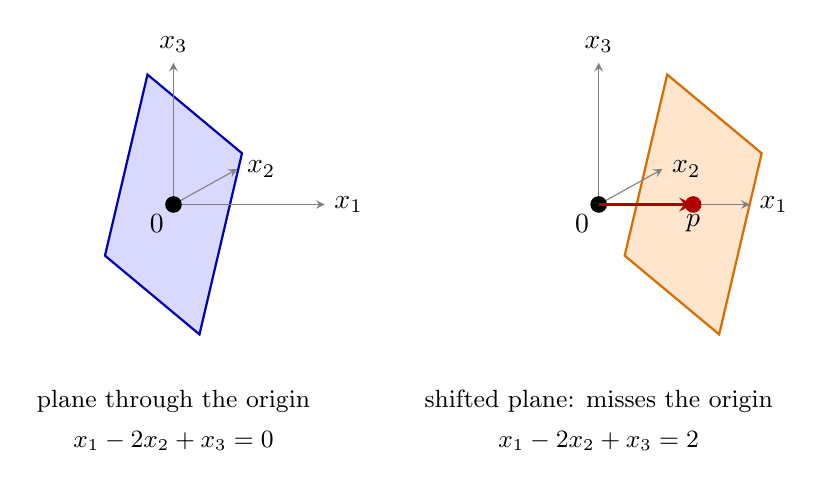
\begin{tikzpicture}[x=0.6cm,y=0.5cm,>=stealth]
  % oblique projection used for both panels: the point (x1,x2,x3) is drawn at (x1+0.45*x2, x3+0.30*x2)
  % plane x1-2x2+x3=0 is spanned by g1=(1,0,-1) and g2=(0,1,2); the patch has corners +-g1+-g2
  \fill[blue!15] (1.45,1.3)--(-0.55,3.3)--(-1.45,-1.3)--(0.55,-3.3)--cycle;
  \draw[thick,blue!70!black] (1.45,1.3)--(-0.55,3.3)--(-1.45,-1.3)--(0.55,-3.3)--cycle;
  \draw[->,gray] (0,0)--(3.2,0);
  \draw[->,gray] (0,0)--(1.35,0.9);
  \draw[->,gray] (0,0)--(0,3.6);
  \node[right] at (3.2,0) {$x_1$};
  \node[right] at (1.35,0.9) {$x_2$};
  \node[above] at (0,3.6) {$x_3$};
  \fill (0,0) circle (3pt);
  \node[below left] at (0,0) {$0$};
  \node at (0,-5.0) {\small plane through the origin};
  \node at (0,-6.0) {\small $x_1-2x_2+x_3=0$};
  \begin{scope}[shift={(9,0)}]
    % shifted plane x1-2x2+x3=2: the same patch moved by p=(2,0,0), drawn at (2,0)
    \fill[orange!20] (3.45,1.3)--(1.45,3.3)--(0.55,-1.3)--(2.55,-3.3)--cycle;
    \draw[thick,orange!85!black] (3.45,1.3)--(1.45,3.3)--(0.55,-1.3)--(2.55,-3.3)--cycle;
    \draw[->,gray] (0,0)--(3.2,0);
    \draw[->,gray] (0,0)--(1.35,0.9);
    \draw[->,gray] (0,0)--(0,3.6);
    \node[right] at (3.2,0) {$x_1$};
    \node[right] at (1.35,0.9) {$x_2$};
    \node[above] at (0,3.6) {$x_3$};
    \fill (0,0) circle (3pt);
    \node[below left] at (0,0) {$0$};
    \draw[->,very thick,red!70!black] (0,0)--(2,0);
    \fill[red!70!black] (2,0) circle (3pt);
    \node[below] at (2,0) {$p$};
    \node at (0,-5.0) {\small shifted plane: misses the origin};
    \node at (0,-6.0) {\small $x_1-2x_2+x_3=2$};
  \end{scope}
\end{tikzpicture}
\end{center}

\textbf{Figure 1.} Left: the plane $H$ of Example~\ref{ex:plane}, a patch drawn in the usual oblique picture of $\R^3$; it passes through the origin. Right: the plane $H_2$ of Example~\ref{ex:shifted}, the same patch moved by the vector $\bv{p}=(2,0,0)$. It is parallel to $H$ and does not contain $\bv{0}$: it is a translate of a subspace, not a subspace.

\begin{exmp}{Four sets that look like nice shapes}{shapes}
\textbf{(a) The first quadrant} $Q=\{(x,y):x\geq0,\ y\geq0\}$. It contains $\bv{0}$ and is closed under addition (sums of nonnegative numbers are nonnegative). But scalars fail: $\bv{u}=(2,1)$ is in $Q$ and $(-1)\bv{u}=(-2,-1)$ is not. Not a subspace.

\textbf{(b) The first and third quadrants} $W=\{(x,y):xy\geq0\}$. It contains $\bv{0}$ and is closed under scalar multiples ($(cx)(cy)=c^2xy\geq0$). But addition fails: $(2,1)$ and $(-1,-2)$ are in $W$, and their sum $(1,-1)$ has $xy=-1<0$. Not a subspace.

\textbf{(c) The two coordinate axes} $L=\{(x,y):xy=0\}$. It contains $\bv{0}$ and is closed under scalar multiples. But $(1,0)$ and $(0,2)$ are in $L$, and $(1,0)+(0,2)=(1,2)$ is not. Not a subspace.

\textbf{(d) The closed unit disk} $D=\{(x,y):x^2+y^2\leq1\}$. It contains $\bv{0}$. But $(1,0)$ and $(0,1)$ are in $D$ and $(1,1)$ is not ($1+1=2>1$), so addition fails; and $\bv{u}=(0.6,0.8)$ is in $D$ ($0.36+0.64=1$) while $2\bv{u}=(1.2,1.6)$ is not ($1.44+2.56=4>1$), so scalars fail as well. Not a subspace.
\end{exmp}

\begin{center}
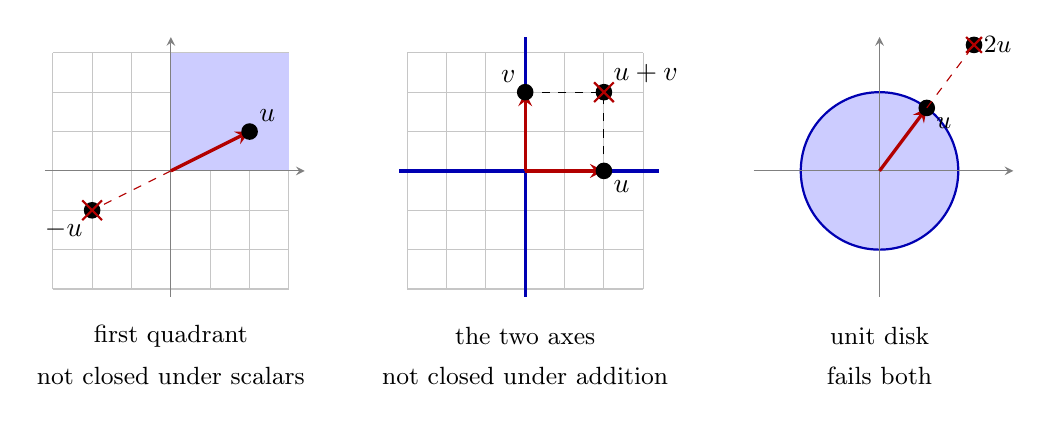
\begin{tikzpicture}[x=0.5cm,y=0.5cm,>=stealth]
  % panel 1: first quadrant, u=(2,1) and (-1)u=(-2,-1)
  \draw[gray!45] (-3,-3) grid[step=1] (3,3);
  \fill[blue!20] (0,0) rectangle (3,3);
  \draw[->,gray] (-3.2,0)--(3.4,0);
  \draw[->,gray] (0,-3.2)--(0,3.4);
  \draw[->,very thick,red!70!black] (0,0)--(2,1);
  \fill (2,1) circle (3pt);
  \node[above right] at (2,1) {$u$};
  \draw[dashed,red!70!black] (0,0)--(-2,-1);
  \fill (-2,-1) circle (3pt);
  \draw[thick,red!70!black] (-2.25,-1.25)--(-1.75,-0.75) (-2.25,-0.75)--(-1.75,-1.25);
  \node[below left] at (-2,-1) {$-u$};
  \node at (0,-4.2) {\small first quadrant};
  \node at (0,-5.2) {\small not closed under scalars};
  \begin{scope}[shift={(9,0)}]
    % panel 2: the two axes, u=(2,0), v=(0,2), u+v=(2,2)
    \draw[gray!45] (-3,-3) grid[step=1] (3,3);
    \draw[very thick,blue!70!black] (-3.2,0)--(3.4,0);
    \draw[very thick,blue!70!black] (0,-3.2)--(0,3.4);
    \draw[->,very thick,red!70!black] (0,0)--(2,0);
    \draw[->,very thick,red!70!black] (0,0)--(0,2);
    \draw[dashed] (2,0)--(2,2)--(0,2);
    \fill (2,0) circle (3pt);
    \fill (0,2) circle (3pt);
    \fill (2,2) circle (3pt);
    \draw[thick,red!70!black] (1.75,1.75)--(2.25,2.25) (1.75,2.25)--(2.25,1.75);
    \node[below right] at (2,0) {$u$};
    \node[above left] at (0,2) {$v$};
    \node[above right] at (2,2) {$u+v$};
    \node at (0,-4.2) {\small the two axes};
    \node at (0,-5.2) {\small not closed under addition};
  \end{scope}
  \begin{scope}[shift={(18,0)},scale=2]
    % panel 3: unit disk drawn with scale 2 (one unit of the disk is 1 cm); u=(0.6,0.8) and 2u=(1.2,1.6)
    \fill[blue!20] (0,0) circle (1);
    \draw[thick,blue!70!black] (0,0) circle (1);
    \draw[->,gray] (-1.6,0)--(1.7,0);
    \draw[->,gray] (0,-1.6)--(0,1.7);
    \draw[->,very thick,red!70!black] (0,0)--(0.6,0.8);
    \fill (0.6,0.8) circle (1.5pt);
    \node[below right] at (0.6,0.8) {\small $u$};
    \draw[dashed,red!70!black] (0.6,0.8)--(1.2,1.6);
    \fill (1.2,1.6) circle (1.5pt);
    \draw[thick,red!70!black] (1.1,1.5)--(1.3,1.7) (1.1,1.7)--(1.3,1.5);
    \node[right] at (1.2,1.6) {\small $2u$};
    \node at (0,-2.1) {\small unit disk};
    \node at (0,-2.6) {\small fails both};
  \end{scope}
\end{tikzpicture}
\end{center}

\textbf{Figure 2.} Three sets that contain the origin but are not subspaces of $\R^2$ (a cross marks a vector outside the set). Left: in the first quadrant, $\bv{u}=(2,1)$ stays inside but $(-1)\bv{u}=(-2,-1)$ does not. Middle: the axes are closed under scalar multiples, but $\bv{u}=(2,0)$ and $\bv{v}=(0,2)$ have the sum $(2,2)$, which is on neither axis. Right (drawn at twice the scale): the unit disk, where $\bv{u}=(0.6,0.8)$ is on the boundary and $2\bv{u}=(1.2,1.6)$ is outside.

\begin{warn}[Nice shapes are not enough]
A set can look like a plane, a quadrant or a disk, pass the zero test, and still fail closure. A subspace must be closed under \emph{both} operations for \emph{all} vectors and \emph{all} scalars, including negative scalars and scalars larger than $1$. A useful picture: if $\bv{u}$ is in a subspace, then the whole line through $\bv{0}$ and $\bv{u}$ is in it, in both directions; and if $\bv{u},\bv{v}$ are in it, so is their sum, and with it the whole plane they span. Half-lines, quadrants and disks violate the first picture, and unions of two lines violate the second.
\end{warn}

\begin{kc}{Subspace or not?}{issub}
Decide whether each set is a subspace, with a one-line reason. (a)~$\{(s,2s,-s):s\in\R\}\subset\R^3$. (b)~$\{(x,y,z):x+y+z=1\}\subset\R^3$. (c)~$\{(x,y):x^2=y^2\}\subset\R^2$. (d)~$\{p\in\mathbb{P}_2:\ p(1)=2p(0)\}$. (e)~$\{A\in M_{2\times2}:\ \det A=1\}$.
\end{kc}

\begin{think}{Why both closure properties?}{both}
Find a subset of $\R^2$ that is closed under addition but not under scalar multiplication, and a subset of $\R^2$ that is closed under scalar multiplication but not under addition. Is it enough to require closure under addition for every \emph{integer} multiple? What do your two examples tell you about the definition of a subspace?
\end{think}

\begin{exmp}{Subspaces of $\mathbb{P}_2$}{polysub}
\textbf{(a)} $H_1=\{p\in\mathbb{P}_2:\ p(0)=0\}$ is a subspace. The zero polynomial has value $0$ at $t=0$. If $p(0)=0=q(0)$, then $(p+q)(0)=p(0)+q(0)=0$ and $(cp)(0)=c\,p(0)=0$. (The polynomials in $H_1$ are those with $a_0=0$, that is, $p(t)=a_1t+a_2t^2$.)

\textbf{(b)} $H_2=\{p\in\mathbb{P}_2:\ p(0)=1\}$ is not a subspace: the zero polynomial has $p(0)=0\neq1$.

\textbf{(c)} $H_3=\{a+t^2:\ a\in\R\}$ is not a subspace. The zero polynomial is not of the form $a+t^2$ (the coefficient of $t^2$ would have to be $1$ and $0$). Closure fails as well: $(1+t^2)+(2+t^2)=3+2t^2$ is not of that form.

\textbf{(d)} $H_4=\{p\in\mathbb{P}_2:\ p\text{ has integer coefficients}\}$ is not a subspace. It contains the zero polynomial and is closed under addition, but $p(t)=1+t$ is in $H_4$ and $\tfrac12p(t)=\tfrac12+\tfrac12t$ is not.
\end{exmp}

\begin{exmp}{Subspaces of $M_{2\times2}$}{matsub}
\textbf{(a) Symmetric matrices.} Let $S=\{A\in M_{2\times2}:\ A\T=A\}$; its elements are the matrices $\begin{bmatrix}a&b\\b&d\end{bmatrix}$. The zero matrix is symmetric. If $A\T=A$ and $B\T=B$, then by Theorem~\ref{2.1-thm:transprops}, $(A+B)\T=A\T+B\T=A+B$ and $(cA)\T=cA\T=cA$. So $S$ is a subspace. For instance $A=\begin{bmatrix}1&2\\2&3\end{bmatrix}$ and $B=\begin{bmatrix}0&-1\\-1&4\end{bmatrix}$ give $A+B=\begin{bmatrix}1&1\\1&7\end{bmatrix}$, again symmetric. The same argument works for symmetric $n\times n$ matrices, for every $n$.

\textbf{(b) Matrices with trace zero.} Let $T=\Bigl\{\begin{bmatrix}a&b\\c&d\end{bmatrix}:\ a+d=0\Bigr\}$. The zero matrix qualifies. If $a+d=0$ and $a'+d'=0$, then $(a+a')+(d+d')=0$, and $ra+rd=0$ for every scalar $r$. So $T$ is a subspace; its elements are the matrices $\begin{bmatrix}a&b\\c&-a\end{bmatrix}$.

\textbf{(c) Invertible matrices} form a set that is \emph{not} a subspace of $M_{2\times2}$: the zero matrix is not invertible, so property (a) fails. (The identity $I$ and $-I$ are invertible and their sum is $\mathbf{0}$.)

\textbf{(d) Singular matrices.} Let $N=\{A\in M_{2\times2}:\ \det A=0\}$. It contains the zero matrix and is closed under scalar multiples, since $\det(cA)=c^2\det A=0$ (Theorem~\ref{3.2-thm:scalar}). But it is not closed under addition: $A=\begin{bmatrix}1&0\\0&0\end{bmatrix}$ and $B=\begin{bmatrix}0&0\\0&1\end{bmatrix}$ are in $N$, and $A+B=I$ has $\det I=1$. Not a subspace.
\end{exmp}

\begin{exmp}{Trivial subspaces, and a chain of subspaces}{chain}
\textbf{The zero subspace.} In any vector space $V$ the set $\{\bv{0}\}$ is a subspace: it contains $\bv{0}$, $\bv{0}+\bv{0}=\bv{0}$ by axiom (4), and $c\bv{0}=\bv{0}$ by Theorem~\ref{thm:conseq}(d). At the other extreme, $V$ itself is a subspace of $V$.

\textbf{A chain.} Let $\mathbb{P}$ be the set of all polynomials of any degree, with the operations of functions. Then $\mathbb{P}_0\subset\mathbb{P}_1\subset\mathbb{P}_2\subset\cdots\subset\mathbb{P}$: each $\mathbb{P}_n$ contains the zero polynomial, and sums and scalar multiples of polynomials of degree at most $n$ have degree at most $n$. The set $\mathbb{P}$ is in turn a subspace of the space of all continuous functions on $\R$ (sums and scalar multiples of continuous functions are continuous, a fact from calculus), which is a subspace of the space $\mathcal{F}$ of all functions on $\R$. Two more subspaces of $\mathcal{F}$: the functions with $f(0)=0$, and the \emph{even} functions, those with $f(-t)=f(t)$ for all $t$. (If $f$ and $g$ are even, then $(f+g)(-t)=f(-t)+g(-t)=f(t)+g(t)=(f+g)(t)$, and likewise for $cf$; the zero function is even.) The set of functions with $f(0)=1$ is not a subspace: the zero function fails.
\end{exmp}

\begin{think}{Intersections and unions}{inter}
Let $H$ and $K$ be subspaces of $V$. (a)~Show that the intersection $H\cap K$ is a subspace of $V$. (b)~Show with an example in $\R^2$ that the union $H\cup K$ need not be a subspace. (c)~Prove that $H\cup K$ is a subspace only if $H\subseteq K$ or $K\subseteq H$. (Hint: suppose neither holds, pick $\bv{u}$ in $H$ but not in $K$ and $\bv{v}$ in $K$ but not in $H$, and ask where $\bv{u}+\bv{v}$ can be.)
\end{think}

\begin{think}{Is $\R^2$ a subspace of $\R^3$?}{r2r3}
A student says, ``The $x_1x_2$-plane is $\R^2$, and it sits inside $\R^3$, so $\R^2$ is a subspace of $\R^3$.'' (a)~Is $\R^2$ a \emph{subset} of $\R^3$? (b)~Let $H=\{(a,b,0):a,b\in\R\}\subset\R^3$. Is $H$ a subspace? (c)~In what sense does $H$ ``look and act like'' $\R^2$, and why is it still wrong to say $H=\R^2$?
\end{think}

% ---------------------------------------------------------------------
\subsection*{Span}

Linear combinations make sense in any vector space, because we can add vectors and multiply them by scalars. Definition~\ref{1.3-def:span} for $\R^n$ now becomes a definition for every $V$.

\begin{defn}{Span of a set of vectors}{span}
Let $\bv{v}_1,\dots,\bv{v}_p$ be vectors in a vector space $V$. The \emph{span} of $\bv{v}_1,\dots,\bv{v}_p$, written $\Span\{\bv{v}_1,\dots,\bv{v}_p\}$, is the set of all linear combinations
\[
c_1\bv{v}_1+c_2\bv{v}_2+\cdots+c_p\bv{v}_p,\qquad c_1,\dots,c_p\text{ real numbers}.
\]
If $H=\Span\{\bv{v}_1,\dots,\bv{v}_p\}$, we say that $H$ is \emph{spanned} (or \emph{generated}) by $\bv{v}_1,\dots,\bv{v}_p$, and that $\{\bv{v}_1,\dots,\bv{v}_p\}$ is a \emph{spanning set} for $H$.
\end{defn}

In Pause and think~\ref{1.3-think:closure} you saw that sums and scalar multiples of linear combinations are again linear combinations. That argument used only the rules of addition and scaling, and so it works in every vector space.

\begin{thm}{A span is a subspace}{spansub}
If $\bv{v}_1,\dots,\bv{v}_p$ are vectors in a vector space $V$, then $\Span\{\bv{v}_1,\dots,\bv{v}_p\}$ is a subspace of $V$.
\end{thm}

\begin{proof}
Let $H=\Span\{\bv{v}_1,\dots,\bv{v}_p\}$. (a)~$\bv{0}=0\bv{v}_1+\cdots+0\bv{v}_p$ by Theorem~\ref{thm:conseq}(c) and axiom (4), so $\bv{0}$ is in $H$. (b)~Let $\bv{u}=s_1\bv{v}_1+\cdots+s_p\bv{v}_p$ and $\bv{w}=t_1\bv{v}_1+\cdots+t_p\bv{v}_p$ be in $H$. By axioms (2), (3) and (8),
\[
\bv{u}+\bv{w}=(s_1+t_1)\bv{v}_1+\cdots+(s_p+t_p)\bv{v}_p,
\]
which is in $H$. (c)~For a scalar $c$, axioms (7) and (9) give $c\bv{u}=(cs_1)\bv{v}_1+\cdots+(cs_p)\bv{v}_p$, which is in $H$.
\end{proof}

The theorem gives a second way to prove that a set is a subspace: write it as a span. The vectors $\bv{v}_1,\dots,\bv{v}_p$ are ``handles'' that let us hold on to the possibly infinite set $H$ with finitely many vectors.

\begin{exmp}{A parametric description is a span}{parametric}
\textbf{(a)} $H=\{(a,\ a+b,\ b):\ a,b\in\R\}\subset\R^3$. Every vector of $H$ is
\[
(a,a+b,b)=a(1,1,0)+b(0,1,1),
\]
so $H=\Span\{(1,1,0),(0,1,1)\}$, and $H$ is a subspace of $\R^3$ by Theorem~\ref{thm:spansub}. Check with $a=2$, $b=-1$: $(2,1,-1)=2(1,1,0)-(0,1,1)=(2,2,0)-(0,1,1)$. \ $\checkmark$

\textbf{(b)} $H=\{(a-3b,\ b-a,\ a,\ b):\ a,b\in\R\}\subset\R^4$. Then
\[
(a-3b,\ b-a,\ a,\ b)=a(1,-1,1,0)+b(-3,1,0,1),
\]
so $H=\Span\{(1,-1,1,0),(-3,1,0,1)\}$ is a subspace of $\R^4$. Check with $a=1$, $b=2$: the vector is $(-5,1,1,2)$ and $(1,-1,1,0)+2(-3,1,0,1)=(-5,1,1,2)$. \ $\checkmark$

\textbf{(c)} The set $\{(1+2s,\ 3s)\}$ has the same form but is not a span: $\bv{0}$ is not in it. The vectors must be \emph{multiplied by the parameters}; a constant vector in the parametric form moves the set off the origin (compare the parametric vector forms of Section 1.5).
\end{exmp}

\begin{exmp}{A restriction can be rewritten as a span}{restriction}
\textbf{(a) In $\R^3$.} Solve the restriction of Example~\ref{ex:plane} for $a$: $a=2b-c$, with $b$ and $c$ free. Then
\[
(a,b,c)=(2b-c,\ b,\ c)=b(2,1,0)+c(-1,0,1),
\]
so $H=\Span\{(2,1,0),(-1,0,1)\}$, exactly as in Example~\ref{1.5-ex:plane} (there the equation was $x_1-2x_2+3x_3=0$). Both vectors satisfy the equation ($2-2+0=0$ and $-1-0+1=0$). The subspace property now comes for free from Theorem~\ref{thm:spansub}.

\textbf{(b) In $\mathbb{P}_2$.} Let $H=\{p\in\mathbb{P}_2:\ p(-1)=0\}$. For $p(t)=a_0+a_1t+a_2t^2$ we have $p(-1)=a_0-a_1+a_2$, so the restriction says $a_0=a_1-a_2$, with $a_1,a_2$ free:
\[
p(t)=(a_1-a_2)+a_1t+a_2t^2=a_1(1+t)+a_2(-1+t^2).
\]
So $H=\Span\{1+t,\ -1+t^2\}$. Check: $1+t$ and $-1+t^2$ vanish at $t=-1$.

\textbf{(c) In $M_{2\times2}$.} The symmetric matrices of Example~\ref{ex:matsub} are
\[
\begin{bmatrix}a&b\\b&d\end{bmatrix}=a\begin{bmatrix}1&0\\0&0\end{bmatrix}+b\begin{bmatrix}0&1\\1&0\end{bmatrix}+d\begin{bmatrix}0&0\\0&1\end{bmatrix},
\]
a span of three matrices. The trace-zero matrices $\begin{bmatrix}a&b\\c&-a\end{bmatrix}$ are
$a\begin{bmatrix}1&0\\0&-1\end{bmatrix}+b\begin{bmatrix}0&1\\0&0\end{bmatrix}+c\begin{bmatrix}0&0\\1&0\end{bmatrix}$, also a span of three matrices.
\end{exmp}

\begin{exmp}{A span of functions}{spanfunc}
A mass on a spring oscillates with a displacement of the form $y(t)=c_1\cos2t+c_2\sin2t$ (the number $2$ is fixed by the spring and the mass; $c_1,c_2$ depend on how the motion starts). The set of all such functions is $H=\Span\{\cos2t,\ \sin2t\}$, a span in the space $\mathcal{F}$ of functions on $\R$. By Theorem~\ref{thm:spansub} it is a subspace of $\mathcal{F}$: a sum of two oscillations of this kind, or a multiple of one, is again an oscillation of this kind.

Is $g(t)=\sin(2t+\tfrac\pi6)$ in $H$? The addition formula gives
\[
\sin\bigl(2t+\tfrac\pi6\bigr)=\sin2t\cos\tfrac\pi6+\cos2t\sin\tfrac\pi6=\tfrac12\cos2t+\tfrac{\sqrt3}{2}\sin2t,
\]
so yes, with $c_1=\tfrac12$ and $c_2=\tfrac{\sqrt3}2$. (Check at $t=0$: $g(0)=\tfrac12$ and $\tfrac12\cdot1+\tfrac{\sqrt3}2\cdot0=\tfrac12$; at $t=\tfrac\pi4$: $g(\tfrac\pi4)=\cos\tfrac\pi6=\tfrac{\sqrt3}2$ and $\tfrac12\cdot0+\tfrac{\sqrt3}2\cdot1=\tfrac{\sqrt3}2$.)

Is $h(t)=\cos t$ in $H$? Suppose $\cos t=c_1\cos2t+c_2\sin2t$ for all $t$. At $t=0$ this says $1=c_1$. At $t=\tfrac\pi2$ it says $0=c_1\cos\pi+c_2\sin\pi=-c_1$. These demands contradict each other, so $h$ is \emph{not} in $H$. Two values of $t$ are enough to rule out membership; to rule it \emph{in}, the equation must hold at every $t$.
\end{exmp}

\begin{kc}{Write it as a span}{aspan}
Show that each set is a subspace by writing it as a span. (a)~$\{(2s+t,\ s-3t,\ 4t):s,t\in\R\}\subset\R^3$. (b)~$\Bigl\{\begin{bmatrix}a&b\\0&a\end{bmatrix}:a,b\in\R\Bigr\}\subset M_{2\times2}$. (c)~$\{(a+b)+2a\,t-b\,t^2:\ a,b\in\R\}\subset\mathbb{P}_2$.
\end{kc}

\begin{think}{The smallest subspace}{smallest}
Let $H$ be any subspace of $V$ that contains the vectors $\bv{v}_1,\dots,\bv{v}_p$. Show that $\Span\{\bv{v}_1,\dots,\bv{v}_p\}$ is contained in $H$. Why does this justify calling the span the \emph{smallest} subspace containing the vectors? How would you use this fact to prove that a given subspace $H$ \emph{equals} $\Span\{\bv{v}_1,\dots,\bv{v}_p\}$?
\end{think}

\begin{exmp}{Find a spanning set, or show that none exists}{layfind}
Each set $W$ is described by two parameters $a,b$. Decide whether $W$ is a subspace; if it is, find a spanning set.

\textbf{(a)} $W_1=\{(a+2b,\ 3a-b,\ 4b)\}$. Split by parameters: $(a+2b,3a-b,4b)=a(1,3,0)+b(2,-1,4)$. So $W_1=\Span\{(1,3,0),(2,-1,4)\}$ is a subspace.

\textbf{(b)} $W_2=\{(2a+1,\ a-b,\ 3b)\}$. Is $\bv{0}\in W_2$? We would need $2a+1=0$, so $a=-\tfrac12$; then $a-b=0$ gives $b=-\tfrac12$; but then $3b=-\tfrac32\neq0$. So $\bv{0}\notin W_2$ and $W_2$ is not a subspace. (There is a constant $1$ in the first entry that cannot come from multiplying a vector by a parameter.)

\textbf{(c)} $W_3=\{(a,\ b,\ ab)\}$. This contains $\bv{0}$, but it is not closed under scalar multiples: $\bv{u}=(1,1,1)$ is in $W_3$ ($a=b=1$), and $2\bv{u}=(2,2,2)$ would need $a=b=2$ and $ab=4\neq2$. The product $ab$ is not a linear expression in the parameters. Not a subspace.
\end{exmp}

% ---------------------------------------------------------------------
\subsection*{Is a vector in a span?}

We now come back to Chapter 1. To decide whether a polynomial, a matrix or a function lies in a span, we write the question as a vector equation, compare coefficients or entries, and obtain a linear system that we can row reduce.

\begin{proc}{Is $\bv{w}$ in $\Span\{\bv{v}_1,\dots,\bv{v}_p\}$?}{member}
\begin{enumerate}
  \item Write $\bv{w}=x_1\bv{v}_1+\cdots+x_p\bv{v}_p$ with unknown weights $x_1,\dots,x_p$.
  \item Compare the two sides: coefficients of $1,t,t^2,\dots$ for polynomials, entries in each position for matrices, values at several $t$ (or an identity valid for all $t$) for functions. For polynomials and matrices this is a system of linear equations in $x_1,\dots,x_p$; its augmented matrix has the coefficient (or entry) lists of $\bv{v}_1,\dots,\bv{v}_p,\bv{w}$ as columns.
  \item Row reduce. If the last column is a pivot column, the system is inconsistent and $\bv{w}$ is \emph{not} in the span. Otherwise it is, and a solution gives the weights (Theorem~\ref{1.2-thm:existuniq}).
\end{enumerate}
\end{proc}

\begin{exmp}{A parameter in a vector of $\R^3$}{memberR3}
For which $h$ is $\bv{y}=(3,1,h)$ in $\Span\{\bv{v}_1,\bv{v}_2\}$, where $\bv{v}_1=(1,0,2)$ and $\bv{v}_2=(-1,1,1)$?

\textbf{Solution.} The augmented matrix has columns $\bv{v}_1,\bv{v}_2,\bv{y}$:
\begin{align*}
\begin{amat}{cc|c}1&-1&3\\0&1&1\\2&1&h\end{amat}
&\rops{R_3-2R_1}
\begin{amat}{cc|c}1&-1&3\\0&1&1\\0&3&h-6\end{amat}
\rops{R_3-3R_2}
\begin{amat}{cc|c}1&-1&3\\0&1&1\\0&0&h-9\end{amat}.
\end{align*}
The system is consistent exactly when $h-9=0$. So $\bv{y}$ is in the span if and only if $h=9$; then $x_2=1$, $x_1=4$, and indeed $4(1,0,2)+(-1,1,1)=(3,1,9)$. \ $\checkmark$
\end{exmp}

\begin{exmp}{Polynomials: a dependent spanning set}{memberP2}
Let $p_1(t)=1+t$, $p_2(t)=t+t^2$, $p_3(t)=1-t^2$ (the polynomials of Example~\ref{1.7-ex:poly}). Which of $q(t)=2+3t+t^2$ and $r(t)=1+t+t^2$ are in $\Span\{p_1,p_2,p_3\}$?

\textbf{Solution.} Record each polynomial by its coefficients of $1,t,t^2$: $p_1\leftrightarrow(1,1,0)$, $p_2\leftrightarrow(0,1,1)$, $p_3\leftrightarrow(1,0,-1)$, $q\leftrightarrow(2,3,1)$, $r\leftrightarrow(1,1,1)$. For $q$:
\begin{align*}
\begin{amat}{ccc|c}1&0&1&2\\1&1&0&3\\0&1&-1&1\end{amat}
&\rops{R_2-R_1}
\begin{amat}{ccc|c}1&0&1&2\\0&1&-1&1\\0&1&-1&1\end{amat}
\rops{R_3-R_2}
\begin{amat}{ccc|c}1&0&1&2\\0&1&-1&1\\0&0&0&0\end{amat}.
\end{align*}
The system is consistent, so $q$ is in the span. The third column is not a pivot column, so $x_3$ is free and the weights are not unique: $x_1=2-x_3$, $x_2=1+x_3$. With $x_3=0$ we get $q=2p_1+p_2$, and indeed $2(1+t)+(t+t^2)=2+3t+t^2$. For $r$:
\begin{align*}
\begin{amat}{ccc|c}1&0&1&1\\1&1&0&1\\0&1&-1&1\end{amat}
&\rops{R_2-R_1}
\begin{amat}{ccc|c}1&0&1&1\\0&1&-1&0\\0&1&-1&1\end{amat}
\rops{R_3-R_2}
\begin{amat}{ccc|c}1&0&1&1\\0&1&-1&0\\0&0&0&1\end{amat}.
\end{align*}
The last row says $0=1$, so $r$ is \emph{not} in the span. This agrees with Example~\ref{ex:restriction}(b): all three polynomials vanish at $t=-1$, so every polynomial in their span does, and $r(-1)=1$. The relation $p_1-p_2-p_3=\bv{0}$ of Example~\ref{1.7-ex:poly} is the reason for the free variable: $p_3$ adds nothing new to the span of $p_1$ and $p_2$.
\end{exmp}

\begin{exmp}{Matrices: a span in $M_{2\times2}$}{memberM}
Let $B_1=\begin{bmatrix}1&1\\0&0\end{bmatrix}$ and $B_2=\begin{bmatrix}0&1\\1&0\end{bmatrix}$. Then $x_1B_1+x_2B_2=\begin{bmatrix}x_1&x_1+x_2\\x_2&0\end{bmatrix}$, so the span consists of the matrices $\begin{bmatrix}p&q\\r&s\end{bmatrix}$ with $s=0$ and $q=p+r$. Decide whether $C=\begin{bmatrix}2&5\\3&0\end{bmatrix}$ and $D=\begin{bmatrix}1&1\\1&0\end{bmatrix}$ are in $\Span\{B_1,B_2\}$.

\textbf{Solution.} List the entries in the order $(1,1),(1,2),(2,1),(2,2)$. For $C$:
\begin{align*}
\begin{amat}{cc|c}1&0&2\\1&1&5\\0&1&3\\0&0&0\end{amat}
&\rops{R_2-R_1}
\begin{amat}{cc|c}1&0&2\\0&1&3\\0&1&3\\0&0&0\end{amat}
\rops{R_3-R_2}
\begin{amat}{cc|c}1&0&2\\0&1&3\\0&0&0\\0&0&0\end{amat}.
\end{align*}
Consistent, with $x_1=2$ and $x_2=3$: $C=2B_1+3B_2$ (check the entry $(1,2)$: $2+3=5$). For $D$:
\begin{align*}
\begin{amat}{cc|c}1&0&1\\1&1&1\\0&1&1\\0&0&0\end{amat}
&\rops{R_2-R_1}
\begin{amat}{cc|c}1&0&1\\0&1&0\\0&1&1\\0&0&0\end{amat}
\rops{R_3-R_2}
\begin{amat}{cc|c}1&0&1\\0&1&0\\0&0&1\\0&0&0\end{amat}.
\end{align*}
The last column is a pivot column: inconsistent, so $D$ is not in the span. This matches the description above: for $D$ we have $q=1$ but $p+r=2$.
\end{exmp}

\begin{kc}{Is it in the span?}{member}
(a)~Is $\bv{w}=(2,1,-3)$ in $\Span\{\bv{v}_1,\bv{v}_2,\bv{v}_3\}$, where $\bv{v}_1=(1,-1,0)$, $\bv{v}_2=(0,1,-1)$, $\bv{v}_3=(1,0,-1)$? How many vectors does the \emph{set} $\{\bv{v}_1,\bv{v}_2,\bv{v}_3\}$ contain, and how many vectors does its \emph{span} contain? (b)~Which of $1+2t+t^2$ and $1+t^2$ are in $\Span\{1+t,\ t+t^2\}$? (c)~Is $\begin{bmatrix}1&2\\2&0\end{bmatrix}$ in the span of the matrices $B_1$ and $B_2$ of Example~\ref{ex:memberM}?
\end{kc}

\subsection*{Summary}
\begin{itemize}
  \item A \textbf{vector space} is a set with an addition and a scalar multiplication satisfying ten axioms (closure, addition, scalar multiplication). $\R^n$, polynomials $\mathbb{P}_n$, matrices $M_{m\times n}$ and functions on an interval are vector spaces. The zero vector is part of the structure and differs from space to space.
  \item From the axioms alone: the zero vector and negatives are unique, $0\bv{u}=\bv{0}$, $c\bv{0}=\bv{0}$ and $(-1)\bv{u}=-\bv{u}$.
  \item To show that something is \emph{not} a vector space, name an axiom that fails and give specific vectors or scalars. Typical failures: closure, no zero vector, a scalar axiom with a modified operation.
  \item A \textbf{subspace} of $V$ is a subset containing $\bv{0}$ and closed under addition and scalar multiplication. By the \textbf{Subspace Test} it is then a vector space, because the other axioms are inherited. Start with the zero vector; it is necessary but not sufficient.
  \item Planes and lines through the origin, the zero subspace and $V$ itself are subspaces; shifted planes, quadrants, disks and unions of lines are not. The intersection of subspaces is a subspace; the union usually is not.
  \item $\Span\{\bv{v}_1,\dots,\bv{v}_p\}$ is always a \textbf{subspace} of $V$. Parametric descriptions are spans, and restrictions can often be rewritten as spans.
  \item To decide whether $\bv{w}$ is in a span, write $\bv{w}=x_1\bv{v}_1+\cdots+x_p\bv{v}_p$, compare coefficients or entries, and row reduce the resulting linear system.
\end{itemize}

\subsection*{Questions to think about before the next section}
\begin{enumerate}
  \item In Sections 1.4 and 1.5 you answered whether the solution set of $A\bv{x}=\bv{0}$ is closed under addition and scalar multiples. What does the Subspace Test now say about that set? Which section of Chapter 1 gave the argument? Section 4.2 will use this observation.
  \item If $H$ and $K$ are subspaces of $V$, is the set $\{\bv{h}+\bv{k}:\bv{h}\in H,\ \bv{k}\in K\}$ of all sums a subspace? If $H$ and $K$ are two different lines through the origin in $\R^2$, what is it?
  \item Can a vector space have exactly two vectors? Can it have exactly one? (Hint: if $\bv{u}\neq\bv{0}$, how many different vectors $c\bv{u}$ are there?)
\end{enumerate}

\subsection*{Answers and discussion}
\begin{description}[leftmargin=0pt,itemsep=5pt]
  \item[Knowledge Check \ref{kc:newworlds}.] (a)~$(2+1)+(1-3)t+(-1+4)t^2=3-2t+3t^2$. (b)~$\begin{bmatrix}3&0\\6&-3\end{bmatrix}-\begin{bmatrix}0&1\\1&1\end{bmatrix}=\begin{bmatrix}3&-1\\5&-4\end{bmatrix}$. (c)~$(f-2g)(t)=1+t-2t^2$; at $t=2$ this is $1+2-8=-5$; and $f(2)-2g(2)=3-2\cdot4=-5$. The same number arises both ways, as the definition of the operations requires.
  \item[Knowledge Check \ref{kc:axiomsteps}.] In order: (A4); (A5); (A3); the hypothesis $\bv{u}+\bv{w}=\bv{v}+\bv{w}$; (A3); (A5); (A4). The equality $\bv{u}+\bv{0}=\bv{u}$ is (A4) read backwards, so the first and the last step are both (A4).
  \item[Knowledge Check \ref{kc:zeroneg}.] (a)~Zero vector: the zero polynomial; $-p(t)=-1+t-2t^3$. (b)~Zero vector: the $2\times3$ zero matrix; $-A=\begin{bmatrix}-1&0&2\\-3&-1&-4\end{bmatrix}$. (c)~Zero vector: the function $z(t)=0$ on $[0,1]$; $(-f)(t)=-t^2$; $(f+(-f))(\tfrac12)=\tfrac14-\tfrac14=0$.
  \item[Knowledge Check \ref{kc:whichaxiom}.] (a)~Not a vector space: axiom (1) fails, since $t^3$ and $1-t^3$ have degree $3$ but their sum $1$ does not (axioms (4) and (6) fail too). (b)~Not a vector space: axiom (6) fails, since $(1,1)$ is in $Q$ but $(-1)(1,1)=(-1,-1)$ is not (so axiom (5) fails as well; closure under addition holds). (c)~Not a vector space: only axiom (10) fails, because $1\odot(2,3)=(2,0)\neq(2,3)$. (Axioms (7), (8), (9) hold: for instance $(c+d)\odot\bv{u}=((c+d)u_1,0)=c\odot\bv{u}+d\odot\bv{u}$.) So axiom (10) is not a consequence of the others. (d)~Not a vector space: axiom (6) fails, since $(1,0)$ has integer entries and $\tfrac12(1,0)=(\tfrac12,0)$ does not (closure under addition holds).
  \item[Knowledge Check \ref{kc:issub}.] (a)~Subspace: $(s,2s,-s)=s(1,2,-1)$ is a span. (b)~Not: $(0,0,0)$ gives $0\neq1$. (c)~Not: $(1,1)$ and $(1,-1)$ satisfy $x^2=y^2$, but their sum $(2,0)$ has $x^2=4\neq0=y^2$. (d)~Subspace: for $p=a_0+a_1t+a_2t^2$ the condition is $a_0+a_1+a_2=2a_0$, i.e.\ $a_1+a_2-a_0=0$, a homogeneous linear equation in the coefficients; the zero polynomial satisfies it, and sums and scalar multiples preserve it exactly as in Example~\ref{ex:plane}. (e)~Not: the zero matrix has determinant $0\neq1$.
  \item[Knowledge Check \ref{kc:aspan}.] (a)~$(2s+t,\ s-3t,\ 4t)$ equals $s(2,1,0)+t(1,-3,4)$, so the set is $\Span\{(2,1,0),(1,-3,4)\}$. (b)~$\begin{bmatrix}a&b\\0&a\end{bmatrix}=a\begin{bmatrix}1&0\\0&1\end{bmatrix}+b\begin{bmatrix}0&1\\0&0\end{bmatrix}$, so it is the span of the two matrices $I$ and $\begin{bmatrix}0&1\\0&0\end{bmatrix}$. (c)~$(a+b)+2at-bt^2=a(1+2t)+b(1-t^2)$, so it is $\Span\{1+2t,\ 1-t^2\}$. Each set is a span, hence a subspace by Theorem~\ref{thm:spansub}.
  \item[Knowledge Check \ref{kc:member}.] (a)~Yes: $2\bv{v}_1+3\bv{v}_2=(2,-2+3,-3)=(2,1,-3)$ (also $\bv{v}_3=\bv{v}_1+\bv{v}_2$, so other weights work). The set has $3$ vectors; its span has infinitely many, because $\bv{v}_1\neq\bv{0}$ and the multiples $c\bv{v}_1$ are all different. (b)~A combination is $a(1+t)+b(t+t^2)=a+(a+b)t+bt^2$. For $1+2t+t^2$: $a=1$, $b=1$, and $a+b=2$ matches, so yes: $(1+t)+(t+t^2)$. For $1+t^2$: $a=1$, $b=1$, but $a+b=2\neq0$, so no. (c)~The matrix has $s=0$, but $q=2$ and $p+r=1+2=3$, so $q\neq p+r$: no. (Row reduction: $x_1=1$, $x_2=2$ from entries $(1,1)$ and $(2,1)$, and then the entry $(1,2)$ would be $3\neq2$.)
  \item[Pause and think \ref{think:used}.] \emph{Rules only:} the argument that a sum of two linear combinations is a linear combination, and the proof that $A(\bv{u}+\bv{v})=A\bv{u}+A\bv{v}$ (Theorem~\ref{1.4-thm:linear}), regroup terms using commutativity, associativity and distributivity and never look at an entry. They could be repeated word for word for polynomials, matrices or functions. \emph{Entries:} row reduction, the row--column rule and parametric vector forms use the entries of vectors in $\R^n$. These are computations; they cannot be repeated in a space where a vector has no entries, unless we first translate the question into $\R^n$, as we did for polynomials in Section 1.7 and will do again below.
  \item[Pause and think \ref{think:prove}.] In $\R^n$, $0\bv{u}=\bv{0}$ is true because $0\cdot u_i=0$ for each entry. In a general space there are no entries, the scalar multiple may be defined by an unusual rule, and all we know are the axioms. In Example~\ref{ex:strange} (scalar multiplication $c\odot(u_1,u_2)=(cu_1,u_2)$) the vector $0\odot(1,1)=(0,1)$ is \emph{not} the zero vector: the ``obvious'' fact is false there, because axiom (8), which is needed to prove it, fails. So the fact is not automatic: it is a consequence of the axioms. Proving it from the axioms once gives it for every vector space at once, including ones we have not met. Moreover it shows that the axioms do their job: they are strong enough to force the elementary algebra that we expect.
  \item[Pause and think \ref{think:function}.] No. The zero vector of the space of functions on $\R$ is the function $z$ with $z(t)=0$ for \emph{every} $t$. The function $f(t)=t$ has $f(0)=0$ at one input only, and $f(1)=1\neq0$. A vector in $\R^3$ needs three numbers; a function has one value for every real $t$, so it takes infinitely many numbers to specify. Two functions are equal only if all their values agree, which is why checking an axiom means checking it at every $t$ (Example~\ref{ex:functions}).
  \item[Pause and think \ref{think:zero}.] (a)~If $H$ is nonempty, take any $\bv{u}$ in $H$; by (c) with $c=0$, $0\bv{u}$ is in $H$, and $0\bv{u}=\bv{0}$ by Theorem~\ref{thm:conseq}(c). So ``nonempty'' implies (a). Conversely (a) shows that $H$ is nonempty. (b)~Yes. In $H$ the vector $\bv{z}$ satisfies $\bv{z}+\bv{z}=\bv{z}$ (axiom (4) in $H$ applied to $\bv{u}=\bv{z}$). In $V$ we also have $\bv{z}+\bv{0}=\bv{z}$. So $\bv{z}+\bv{z}=\bv{z}+\bv{0}$, and the cancellation law of Knowledge Check~\ref{kc:axiomsteps} gives $\bv{z}=\bv{0}$. A subspace cannot have its own, different zero vector: it shares the zero vector of $V$. (c)~If $\bv{0}$ is not in $H$ the test is over at once, with no computation of closure. Many subsets fail only this test, such as shifted planes and lines that miss the origin.
  \item[Pause and think \ref{think:both}.] \emph{Closed under addition, not scalars:} the vectors of $\R^2$ with integer entries, or the first quadrant. \emph{Closed under scalars, not addition:} the union of the two coordinate axes, or the set $\{xy\geq0\}$ (Example~\ref{ex:shapes}). Closure under addition gives all positive-integer multiples $\bv{u}+\bv{u}$, $\bv{u}+\bv{u}+\bv{u}$, \dots, and (with a zero vector and negatives) all integer multiples, but not $\tfrac12\bv{u}$: the integer vectors show that this is not enough. Closure under scalars alone only gives the line through $\bv{0}$ and $\bv{u}$ for each $\bv{u}$; the union of two lines shows that sums of vectors from different lines can escape. The two properties control different things (``stay on the line through the origin'' and ``stay in the set when moving in two directions''), and a subspace needs both.
  \item[Pause and think \ref{think:inter}.] (a)~$\bv{0}$ is in both $H$ and $K$, hence in $H\cap K$. If $\bv{u},\bv{v}$ are in $H\cap K$, then $\bv{u}+\bv{v}$ is in $H$ (since $H$ is closed) and in $K$ (since $K$ is closed), so it is in $H\cap K$; the same argument works for $c\bv{u}$. (b)~Let $H$ and $K$ be the $x_1$-axis and the $x_2$-axis (subspaces of $\R^2$). The union is the set $L$ of Example~\ref{ex:shapes}(c), which is not closed under addition: $(1,0)+(0,2)=(1,2)$. (c)~Suppose $\bv{u}\in H$, $\bv{u}\notin K$, and $\bv{v}\in K$, $\bv{v}\notin H$. If $\bv{u}+\bv{v}$ were in $H$, then $\bv{v}=(\bv{u}+\bv{v})+(-\bv{u})$ would be in $H$, a contradiction. If $\bv{u}+\bv{v}$ were in $K$, then $\bv{u}=(\bv{u}+\bv{v})+(-\bv{v})$ would be in $K$, a contradiction. So $\bv{u}+\bv{v}$ is in neither, hence not in $H\cup K$, and the union is not closed under addition. Hence if $H\cup K$ is a subspace, one of $H,K$ contains the other.
  \item[Pause and think \ref{think:r2r3}.] (a)~No. The vectors of $\R^2$ have two entries and those of $\R^3$ have three; $(1,2)$ is not an element of $\R^3$. (b)~Yes: $(0,0,0)$ is in $H$, and adding or scaling vectors with third entry $0$ gives a vector with third entry $0$. (c)~$H$ ``looks and acts like'' $\R^2$ because $(a,b,0)+(a',b',0)=(a+a',b+b',0)$ and $c(a,b,0)=(ca,cb,0)$: the arithmetic of $H$ is that of $\R^2$ with an extra entry $0$ carried along. But the \emph{objects} are different (lists of three numbers versus lists of two). It is correct to say that $H$ is a subspace of $\R^3$ that behaves like $\R^2$, and wrong to say $H=\R^2$.
  \item[Pause and think \ref{think:smallest}.] Each vector $c_1\bv{v}_1+\cdots+c_p\bv{v}_p$ of the span is built from vectors $\bv{v}_i$ in $H$ by scalar multiplication and addition, and $H$ is closed under both. So it is in $H$. Thus any subspace containing the $\bv{v}_i$ contains the span, which is itself a subspace containing the $\bv{v}_i$ (Theorem~\ref{thm:spansub}): the span is the smallest. To prove $H=\Span\{\bv{v}_1,\dots,\bv{v}_p\}$ for a given subspace $H$, prove two inclusions: each $\bv{v}_i$ is in $H$ (so the span is inside $H$), and each vector of $H$ is a linear combination of the $\bv{v}_i$ (so $H$ is inside the span). In Example~\ref{ex:restriction}(a) the second inclusion is the computation $(a,b,c)=b(2,1,0)+c(-1,0,1)$ and the first is the check that both vectors satisfy the equation.
  \item[Before the next section.] (1)~By Theorem~\ref{1.4-thm:linear}, if $A\bv{u}=\bv{0}$ and $A\bv{v}=\bv{0}$ then $A(\bv{u}+\bv{v})=\bv{0}$ and $A(c\bv{u})=\bv{0}$; also $A\bv{0}=\bv{0}$. So the solution set of $A\bv{x}=\bv{0}$ is a subspace of $\R^n$; Section 1.5 also wrote it as a span of the vectors that multiply the free variables (Example~\ref{1.5-ex:hom2}). (2)~Yes: $\bv{0}=\bv{0}+\bv{0}$ is a sum; $(\bv{h}+\bv{k})+(\bv{h}'+\bv{k}')=(\bv{h}+\bv{h}')+(\bv{k}+\bv{k}')$ and $c(\bv{h}+\bv{k})=c\bv{h}+c\bv{k}$. For two different lines through the origin in $\R^2$ it is all of $\R^2$, because the parallelogram rule reaches every point. Note that the union of the two lines is \emph{not} a subspace (Pause and think~\ref{think:inter}); the set of all sums is. (3)~One vector: yes, $\{\bv{0}\}$ is a vector space. Exactly two: no. A space with a vector $\bv{u}\neq\bv{0}$ has infinitely many vectors: if $c\bv{u}=d\bv{u}$ with $c\neq d$, then $(c-d)\bv{u}=\bv{0}$, and multiplying by $\tfrac1{c-d}$ gives $\bv{u}=\tfrac1{c-d}\bv{0}=\bv{0}$ (Theorem~\ref{thm:conseq}(d)), a contradiction. So the multiples $c\bv{u}$ are all different. Hence every vector space has one vector or infinitely many; never exactly two.
\end{description}

\end{document}
